\documentclass[t]{beamer}


\mode<presentation>
{
  \usetheme{Boadilla}  
  \usecolortheme{default} 
  \usefonttheme{default}  
  \setbeamertemplate{navigation symbols}{}
  \setbeamertemplate{caption}[numbered]
} 

\usepackage[slovene]{babel}
\usepackage[utf8]{inputenc}
\usepackage{pgfplots}
\usepackage{listings}
\usepackage{cancel}

\title{Občutljivost optimalne rešitve celoštevilskega linearnega programa}

\author
{Laura Štangelj \and Jakov Kavčič}
\date{2017}

\pgfplotsset{compat=1.12}

\begin{document}

\begin{frame}
  \titlepage
\end{frame}

\begin{frame}{Opis problema in način reševanja}
$$\min\left\{f^Tx; Ax \leq b, 1000 \geq x \geq 1, x \in \mathbb{Z}^n \right\}$$
\begin{itemize}
\item Fiksiramo matriko $A$
\item Opazujemo občutljivost optimalne rešitve, glede na spremembe koeficientov $f$ in $b$.
\item Odločila sva se opazovati štiri razsežne programe.
\end{itemize}
\end{frame}

\begin{frame}
\frametitle{Način reševanja}
\begin{center}
$b = \begin{bmatrix}
b_1\\
b_2\\
b_3\\
b_4\\
\end{bmatrix}$, $f = \begin{bmatrix}
f_1\\
f_2\\
f_3\\
f_4\\
\end{bmatrix}$
\end{center}
\begin{itemize}
\item Spreminjamo le en koeficient vektorja
\item Opazovala sva če se spremeni optimalna rešitev ali vrednost
\item Primerjala sva rezultate z originalno optimalno rešitvijo
\end{itemize}
\end{frame}


\begin{frame}
\frametitle{Način reševanja}
\begin{itemize}
\item Izbrala sva Matlab
\item Za reševanje posameznega CLP sva uporabila funkcijo $intlinprog$
\item Funkcija je programe reševala z dual simplex metodo
\end{itemize}
\end{frame}

\lstset{language=Matlab} 
\begin{lstlisting}
Y=[];
h=1;
for i=1:4
     j=1;
     o=b(i);
     for n=1:s
          db=-10+20*rand();
          b(i)=b(i)+db;
          [x,fval]=intlinprog(f,intcon,A,b,Ae,be,[sp],[zg],options);
          B(i,j)=fval;
          B(i,j+1)=db;
          Y(:,h)=x;
          h=h+1;
	j=j+2;
	b(i)=o;
     end
end
\end{lstlisting}

\begin{frame}{Spremenljivke}
\begin{itemize}
\item $f$ - namenski vektor, ki opisuje namensko funkcijo
\item $b$ - omejitveni vektor
\item $A$ - na začetku definirana matrika
\item $df$ oz. $db$ - motnji koeficientov
\item $x$ - optimalno rešitev
\item $fval$ - optimalna vrednost
\item $intcon$ - vektor, ki določa celoštevilnost rešitve
\item $s$ - število iteracij
\item $sm$ oz. $zm$ - spodnja in zgornja meja
\item $X$ oz. $Y$ - matriki v katerih so shranjene optimalne rešitve
\item $F$ oz. $B$ - matriki v katerih so shranjene optimalne vrednosti in motnje
\end{itemize}
\end{frame}

\begin{frame}{Analiza občutljivosti CLP velikosti $4x4$}
\begin{center}
Poiskala sva dva zanimiva programa na katerih smo izvajali poskuse in tudi analizirala rezultate:
\begin{itemize}
\item CLP-1 - vpliva omejitvenega vektorja
\item CLP-2 - vpliv namenske funkcije
\end{itemize}
\end{center}
\end{frame}

\begin{frame}{CLP-1}
\begin{center}
$ A = \begin{bmatrix}
  1 & -2 & 3 & 4 \\
  9 & -3 & 4 & 5 \\
  1 & -3 & 5 & 7 \\
  2 & -4 & -5 & 1  
\end{bmatrix} $, $f=\begin{bmatrix} 10 \\10 \\10\\10 \end{bmatrix}$, $b=\begin{bmatrix} 12 \\12 \\12\\12 \end{bmatrix}.$
\end{center}
\begin{itemize}
\item Naredila sva 40 iteracij
\item Določila sva interval na katerem naključno izbiramo $df \in (-10,10)$ oz. $db \in (-10,10)$
\end{itemize}
\end{frame}

\begin{frame}{CLP-1}
\begin{figure}[h]
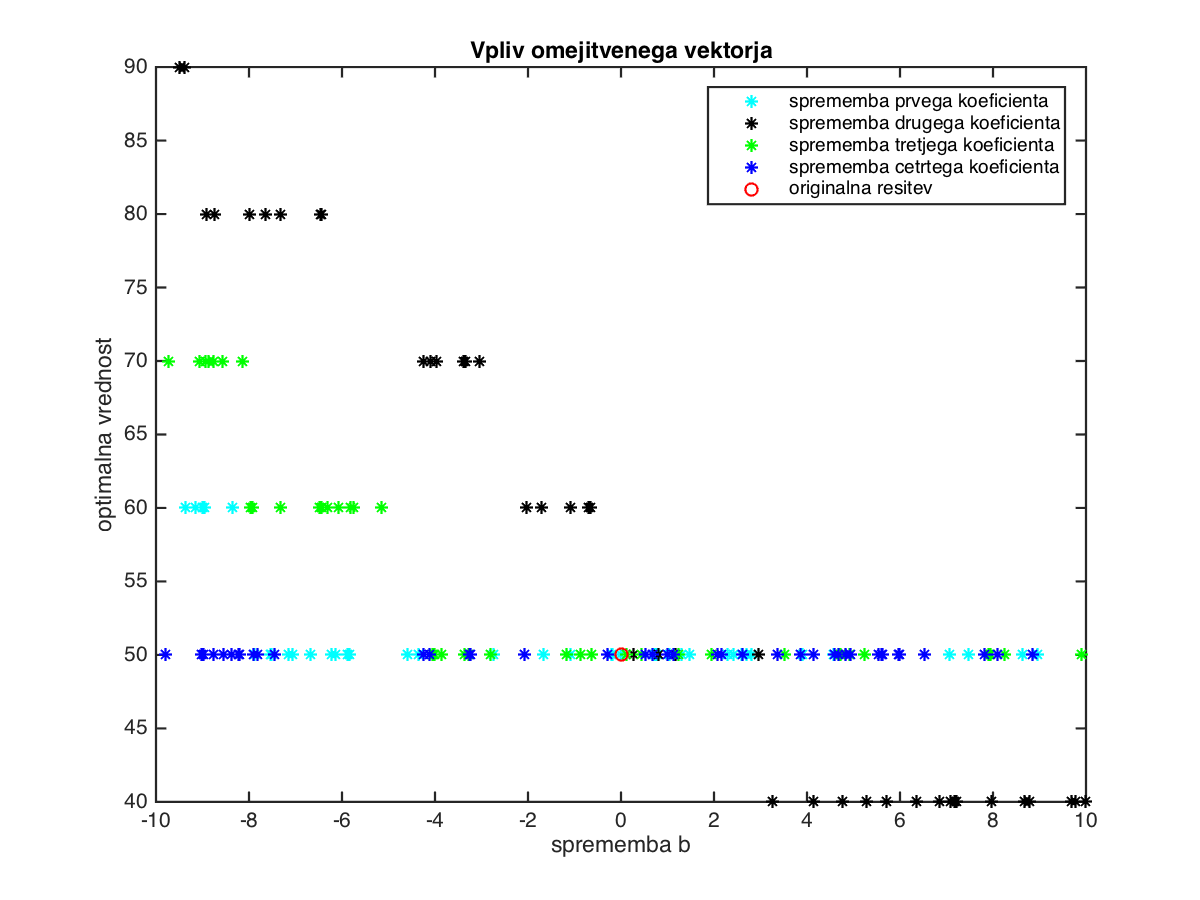
\includegraphics[width=11.2cm,height=8cm]{spremembe_b.png}
\end{figure}
\end{frame}

\begin{frame}{CLP-1}
\begin{figure}[h]
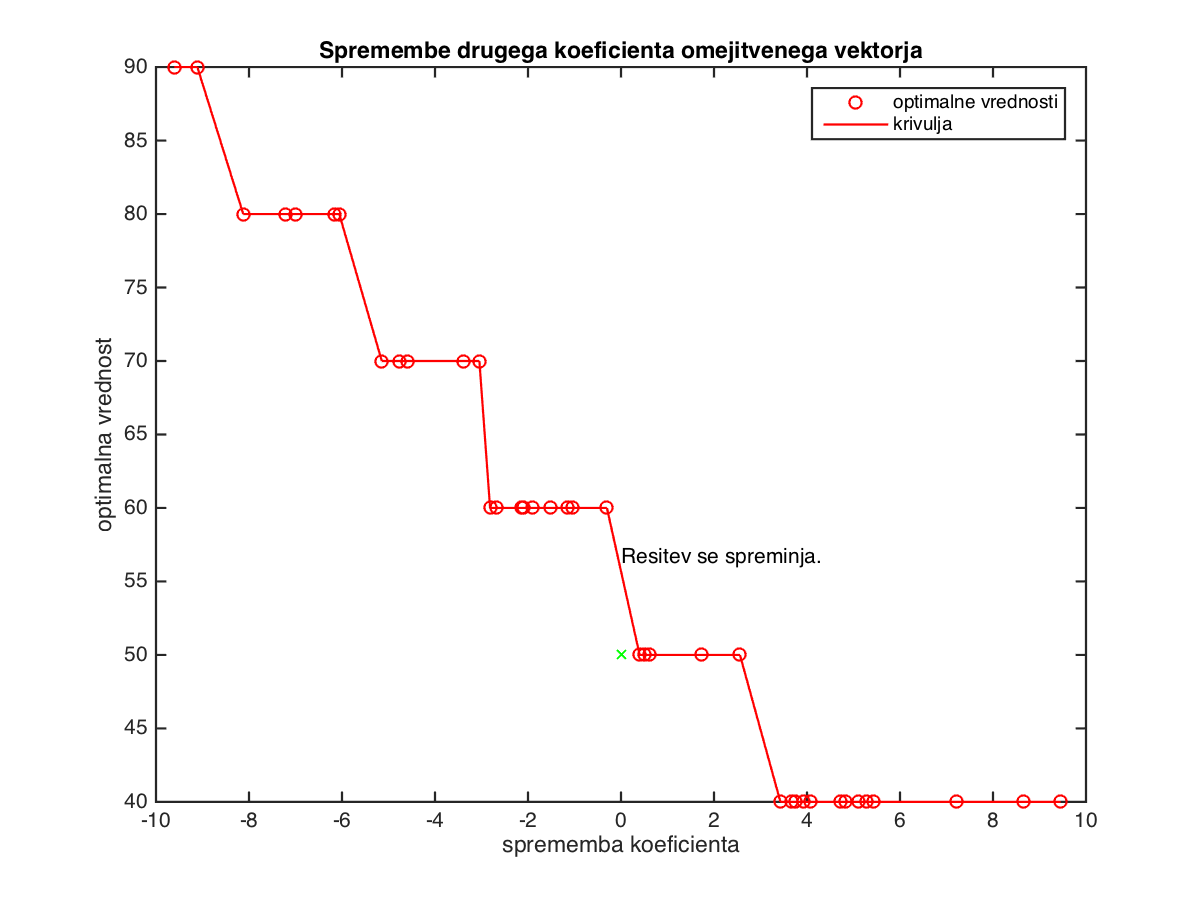
\includegraphics[width=11.2cm,height=8cm]{spremembe_b2.png}
\end{figure}
\end{frame}

\begin{frame}{CLP-2}
\begin{center}
$ A = \begin{bmatrix}
  2 & 6 & -3 & -3 \\
  2 & 4 & 1 & -1 \\
  -4 & -7 & -4 & -5 \\
   7 & -3 & -4 & -5  
\end{bmatrix} $, $f=\begin{bmatrix} -10 \\-10 \\-10\\ -10 \end{bmatrix}$, $b=\begin{bmatrix} 12 \\12 \\-12\\12 \end{bmatrix}.$
\end{center}
\begin{itemize}
\item Naredila sva 40 iteracij
\item Določila sva interval na katerem naključno izbiramo $df \in (-10,10)$ oz. $db \in (-10,10)$
\item Podrobneje sva pogledala, kaj se dogaja z optimalno vrednostjo ko spreminjamo tretji koeficient namenske funkcije za $df \in (4.5,5.5)$ 
\end{itemize}
\end{frame}

\begin{frame}{CLP-2}
\begin{figure}[h]
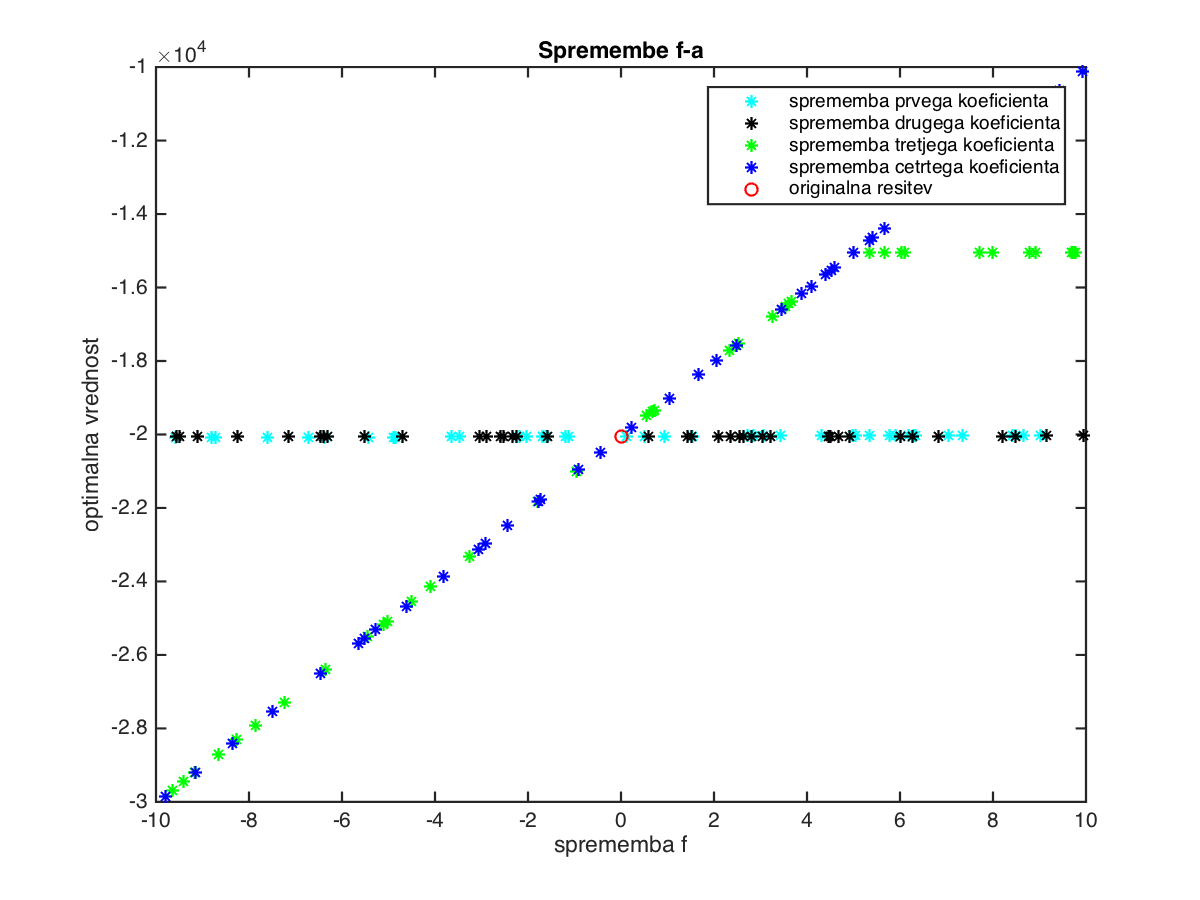
\includegraphics[width=11.2cm,height=8cm]{spremembe_f.png}
\end{figure}
\end{frame}

\begin{frame}{CLP-2}
\begin{figure}[h]
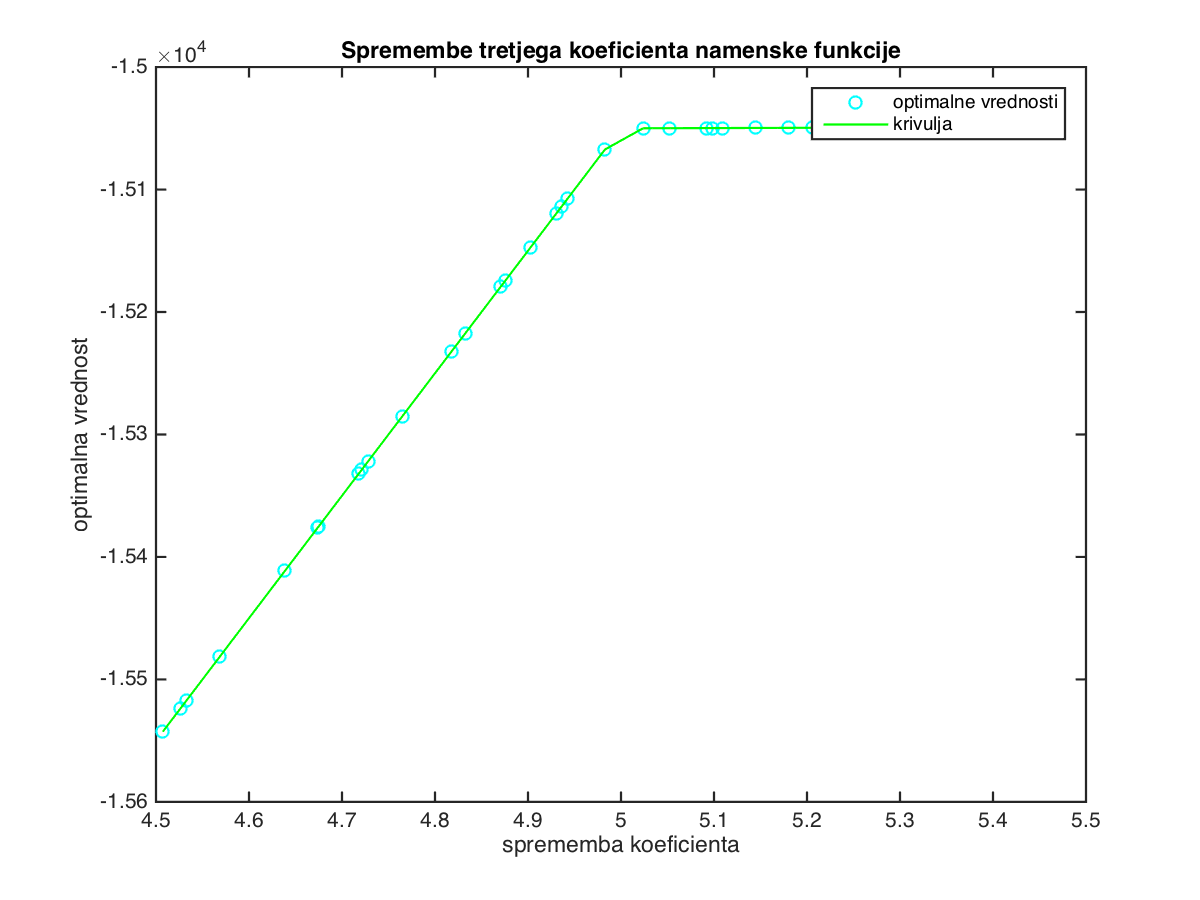
\includegraphics[width=11.2cm,height=8cm]{spremembe_f3.png}
\end{figure}
\end{frame}

\begin{frame}{CLP-2}
\begin{figure}[h]
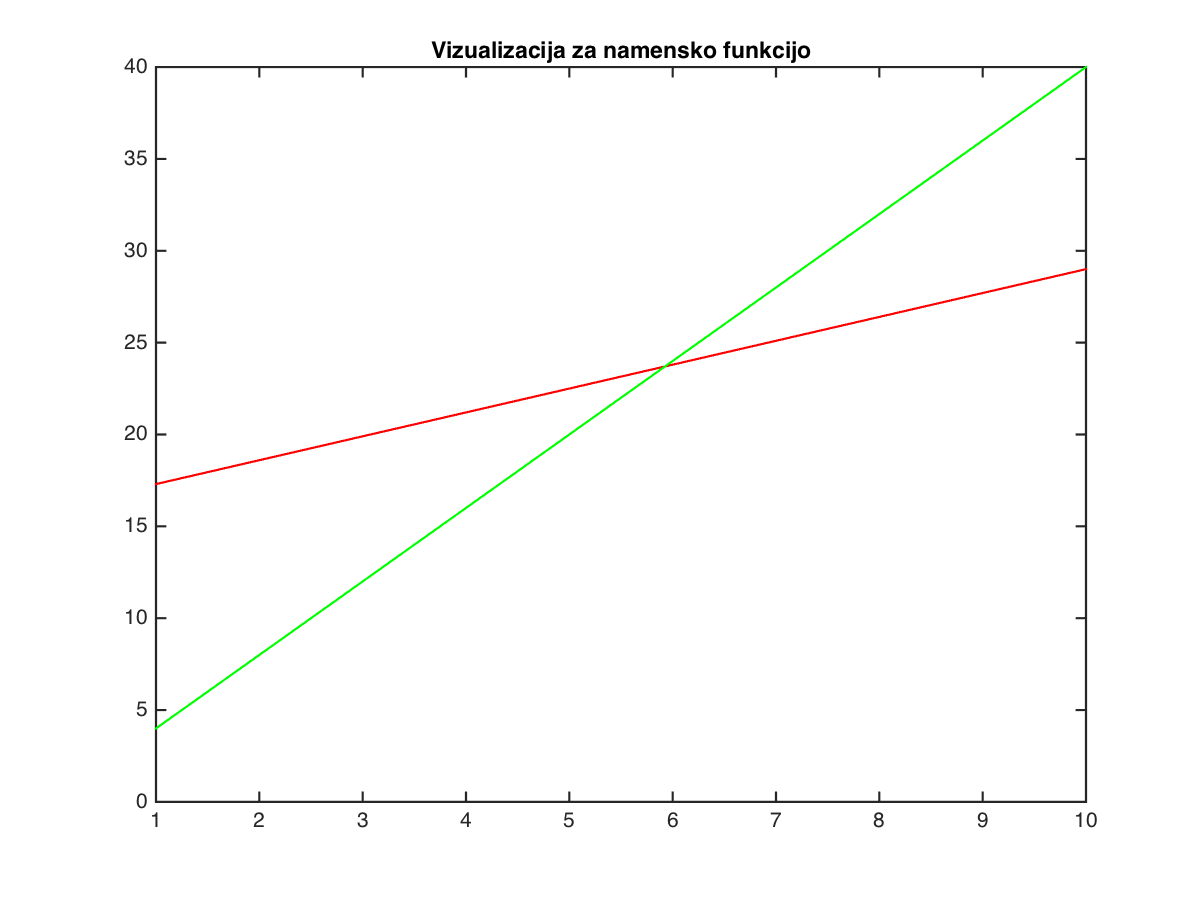
\includegraphics[width=11.2cm,height=8cm]{razlaga1.png}
\end{figure}
\end{frame}


\begin{frame}{Vizualizacija občutljivosti celoštevilskega linearnega programa}
\begin{center}
Za boljšo vizualizacijo učinkov namenskega in omejitvenega vektorja, sva analizirala celoštevilski linearni program velikosti $2x2$
\\[0.5cm]
$ A = \begin{bmatrix}
  -3 & 1  \\
  2 & 1   
\end{bmatrix} $, $f=\begin{bmatrix} -4 \\ 6\end{bmatrix}$, $b=\begin{bmatrix} 3 \\ 10 \end{bmatrix}.$
\end{center}
\end{frame}

\begin{frame}{Vpliv omejitvenega vektorja}
\begin{center}
\begin{figure}[h]
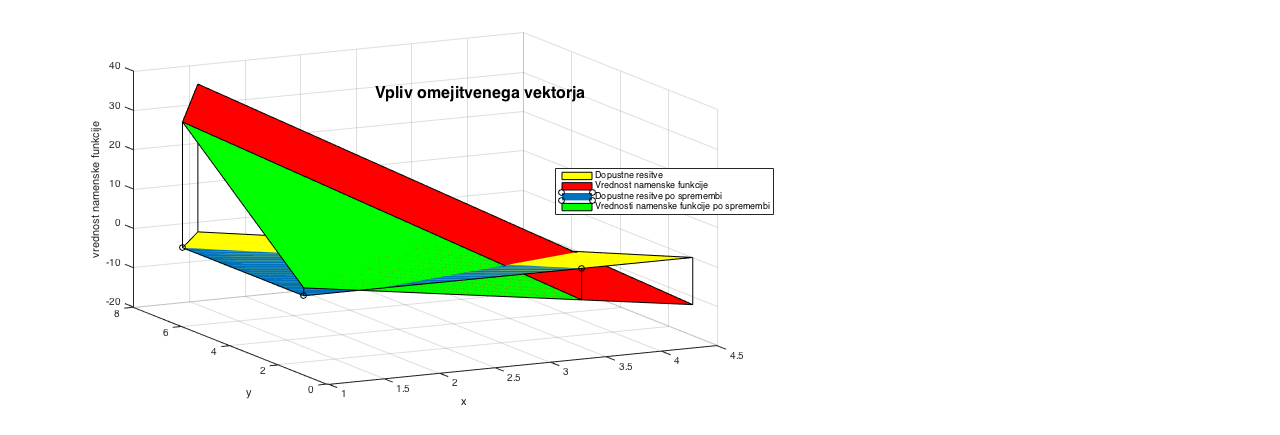
\includegraphics[width=9.1cm,height=6.5cm]{viz1.png}
\end{figure}
$b=\begin{bmatrix} 3 \\ 10 \end{bmatrix} \to b=\begin{bmatrix} 3 \\ 8\end{bmatrix} \Rightarrow x=\begin{bmatrix} 4 \\ 1 \end{bmatrix} \to x=\begin{bmatrix} 3 \\ 1\end{bmatrix} , f^T*x=-10 \to f^T*x=-6$
\end{center}
\end{frame}

\begin{frame}{Vpliv namenskega vektorja}
\begin{center}
\begin{figure}[h]
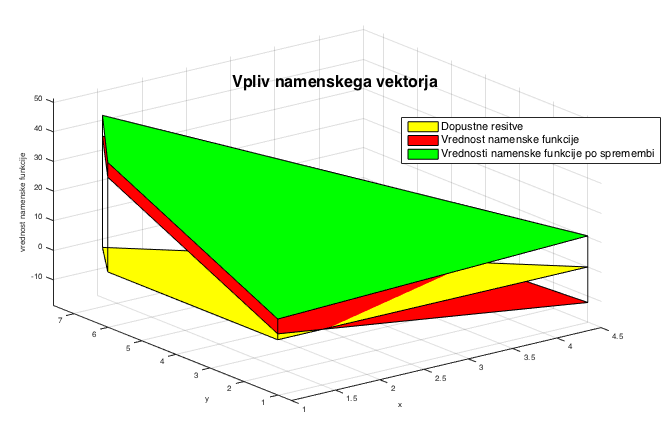
\includegraphics[width=9.1cm,height=6.5cm]{viz2.png}
\end{figure}
$b=\begin{bmatrix} 3 \\ 10 \end{bmatrix} \to b=\begin{bmatrix} 3 \\ 8\end{bmatrix} \Rightarrow x=\begin{bmatrix} 4 \\ 1 \end{bmatrix} \to x=\begin{bmatrix} 3 \\ 1\end{bmatrix}, f^T*x=-10 \to f^T*x=7$
\end{center}
\end{frame}

\end{document}


